%!TEX root = ../template.tex
%%%%%%%%%%%%%%%%%%%%%%%%%%%%%%%%%%%%%%%%%%%%%%%%%%%%%%%%%%%%%%%%%%%
%% chapter4.tex
%% UNIPD thesis document file
%%
%% Chapter with introduction
%%%%%%%%%%%%%%%%%%%%%%%%%%%%%%%%%%%%%%%%%%%%%%%%%%%%%%%%%%%%%%%%%%%

\typeout{NT FILE chapter4.tex}%

\chapter{Reti neurali artificiali per la previsione del gradimento alimentare}
\label{cha:chapter4}
\prependtographicspath{{Chapters/Figures/Covers/}}

\section{Introduzione alle reti neurali artificiali nel contesto della previsione del gradimento alimentare}

Le \gls{ann} sono strumenti sempre più utilizzati per analizzare fenomeni complessi, soprattutto quando variabili interdipendenti e non lineari influenzano i risultati. In ambito ristorativo, il rumore di fondo può avere un impatto significativo sull'esperienza gustativa e sul gradimento del cibo.

Studi precedenti hanno dimostrato che sia le caratteristiche acustiche, come il tipo e il livello del rumore, sia i fattori individuali, come età e sensibilità al rumore, possono influenzare la percezione del gusto. Tuttavia, il peso specifico di ciascuno di questi fattori sul gradimento alimentare in ambienti rumorosi non è ancora del tutto chiaro.

Questo capitolo esplora l'impiego delle reti neurali ottimizzate con l'algoritmo \gls{hho} per migliorare le previsioni sul gradimento del cibo in presenza di rumore di fondo, proponendo un approccio che mira a superare le prestazioni dei modelli statistici tradizionali.

\begin{figure}[H]
    \centering
    
\includegraphics[width=0.5\textwidth]{Chapters/Figures/brain.png}
    \caption{\small Brain neural network. \cite{neural2024}}
    \label{fig:brain}
\end{figure}

Le \gls{ann} offrono vantaggi significativi nell'ambito della previsione del gradimento alimentare, in particolare per la loro capacità di modellare relazioni non lineari. Grazie alla loro struttura, le ANN riescono a catturare e rappresentare relazioni complesse tra variabili di input e output senza richiedere assunzioni preliminari sulla forma di queste relazioni. Ad esempio, possono modellare come la combinazione del livello sonoro e della sensibilità personale al rumore influisca sul gradimento del cibo in un ristorante affollato, un fenomeno difficilmente descrivibile con modelli lineari tradizionali. Questa flessibilità si rivela particolarmente importante per comprendere preferenze alimentari influenzate da interazioni sensoriali complesse. \cite{PANAGOU2009121}

Un altro punto di forza delle reti neurali è la loro abilità nel gestire dati multidimensionali. La capacità di processare ed elaborare simultaneamente molteplici variabili di input permette alle \gls{ann} di analizzare informazioni provenienti da fonti diverse, come fattori acustici, caratteristiche individuali e parametri ambientali. Ad esempio, in una previsione di gradimento alimentare, una ANN può considerare contemporaneamente dati come il tipo di rumore di fondo (musica, traffico, conversazioni), il volume del rumore, e variabili demografiche del cliente (come età e genere). Questi elementi combinati permettono di costruire una previsione accurata che riflette meglio l'esperienza soggettiva dell'utente. \cite{YU201868}

Inoltre, le reti neurali possiedono una notevole capacità di apprendimento adattivo, che consente loro di migliorare continuamente le proprie prestazioni predittive con l'introduzione di nuovi dati. Ad esempio, un modello di \gls{ann} può essere aggiornato in tempo reale con dati raccolti da sensori ambientali o feedback dei clienti, permettendogli di adattarsi alle variazioni delle preferenze nel corso del tempo e migliorando le raccomandazioni di gradimento. Tale adattabilità le rende strumenti estremamente flessibili e ideali per ambienti dinamici dove le condizioni acustiche possono cambiare durante la giornata.

Un aspetto rilevante delle \gls{ann} è la loro robustezza nell'elaborazione di dati rumorosi o incompleti. Questa caratteristica è particolarmente preziosa nelle applicazioni che richiedono valutazioni soggettive, in cui la variabilità naturale delle risposte umane e l'influenza di fattori esterni non controllabili rappresentano elementi di disturbo. Per esempio, in una situazione in cui le risposte dei clienti al gradimento del cibo sono influenzate da fattori imprevisti (come uno stato d'animo negativo o un'interazione sociale durante il pasto), le ANN riescono comunque a identificare pattern affidabili grazie alla loro capacità di generalizzare dai dati imperfetti. \cite{krishnamurthy2022}

Le \gls{ann} hanno dimostrato la loro efficacia in diversi ambiti della valutazione alimentare, come la previsione delle valutazioni dell'appetito. Tuttavia, prima dello studio presentato in \cite{alamir2021enhanced}, non erano mai state applicate alla previsione dell'apprezzamento del cibo in presenza di rumore di fondo, nonostante la loro comprovata superiorità rispetto ai modelli statistici tradizionali nel gestire relazioni non lineari. Questa caratteristica è particolarmente rilevante nel contesto dell'esperienza gastronomica, dove la relazione tra stimoli acustici e percezione del gusto presenta evidenti non linearità che i modelli statistici classici faticano a catturare.

L'utilizzo delle \gls{ann} in questo campo apre nuove frontiere per comprendere e prevedere come diversi fattori ambientali, in particolare il rumore, influenzano l'esperienza gastronomica. Questa comprensione non solo ha implicazioni pratiche per l'industria della ristorazione, ma offre anche preziosi spunti sulle complesse interazioni tra i nostri sensi nella percezione del cibo. La ricerca proposta mira a esplorare e quantificare queste interazioni attraverso l'implementazione di un modello \gls{ann} avanzato, con l'obiettivo di fornire uno strumento predittivo accurato e versatile per l'ottimizzazione dell'esperienza culinaria in diversi ambienti acustici.

\section{Architettura delle ANN}
\noindent

Le \gls{ann} si basano su un'architettura \gls{mlp} progettata per predire il gradimento del cibo in presenza di rumori di sottofondo. La struttura è stata attentamente organizzata in tre componenti principali che lavorano in sinergia per elaborare e analizzare i dati.

La configurazione della rete inizia con uno strato di input, composto da cinque neuroni, ciascuno corrispondente a un particolare fattore che si presume influenzi la percezione del gradimento alimentare in un ambiente rumoroso. Questi fattori includono l'età e il genere del soggetto, la sensibilità personale al rumore, il tipo di rumore presente e il livello di rumore. Ogni neurone nello strato di input riceve informazioni relative a uno di questi parametri, fornendo una base dettagliata per l'analisi predittiva della rete.
    
Segue una serie di strati nascosti, progettati per svolgere un'elaborazione più profonda delle informazioni. Nella rete proposta sono presenti due strati nascosti, ciascuno contenente dieci neuroni. Per massimizzare la capacità della rete di gestire relazioni non lineari complesse, è stata utilizzata una funzione di attivazione \gls{tanh} all'interno di questi strati. Le connessioni tra i neuroni sono unidirezionali, con pesi variabili tra -1 e 1, consentendo alla rete di adattare l'importanza relativa di ogni connessione in base al contesto specifico dei dati.

Infine, tutte le informazioni elaborate negli strati nascosti vengono convogliate nello strato di output, dove una funzione di attivazione lineare genera il risultato finale: una previsione del gradimento alimentare in diverse condizioni sonore. L'output prodotto da questa architettura rappresenta una valutazione che riflette quanto il cibo viene apprezzato in funzione dei diversi livelli e tipi di rumore presenti nell'ambiente.

\begin{figure}[H]
      \centering
      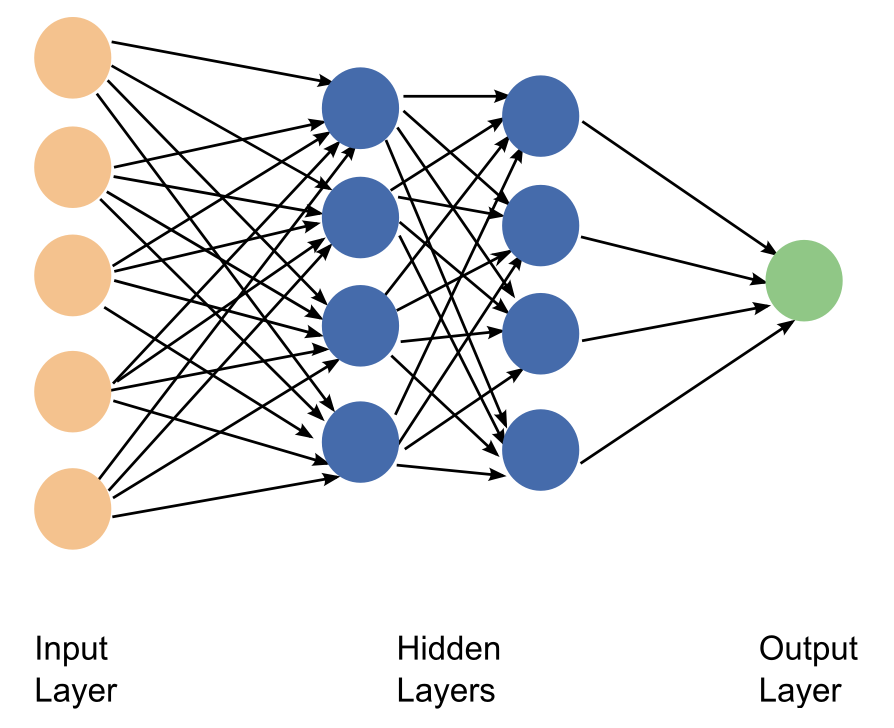
\includegraphics[width=0.6\textwidth]{Chapters/Figures/ArchitectureANN.png}
      \caption{\small Architettura delle reti neurali. Lo strato di ingresso contiene fattori predittivi, mentre lo strato di uscita contiene le valutazioni di gradimento dei cibi. Gli strati sovrapposti o gli strati nascosti hanno un certo numero di neuroni. \cite{alamir2021enhanced}}
      \label{fig:architectureann}
  \end{figure}

  L'output di ciascuno layer l è dato dalla formula:

\begin{equation}
  O_i^{(l)} = \varphi(u_i^{(l)}) = \varphi(\sum_{j=1}^{nl} O_j^{(l-1)} w_{ji}^{(l)} + w_{0,i}^{(l)}), 1 \le l \le L
\end{equation}
  dove $u$ è la funzione di attivazione (solitamente una funzione \gls{tanh} non lineare per gli strati nascosti e una funzione lineare per lo strato di output), $l$ è l'indice dello strato, $w_{j,i}^{(l)}$ sono i pesi delle interconnessioni tra i neuroni, e $w_{0,i}^{(l)}$ sono i bias dei neuroni.

  Questa architettura \gls{mlp} con connessioni bidirezionali tra gli strati è stata utilizzata per modellare la complessità delle relazioni tra i fattori di ingresso e la gradevolezza relativa del cibo.

\begin{comment}
La scelta di questa architettura è stata motivata da una serie di considerazioni:

\begin{itemize}
    \item \textbf{Complessità del problema}: I due strati nascosti permettono alla rete di catturare relazioni non lineari complesse tra gli input e l'output.
    
    \item \textbf{Bilanciamento tra complessità e generalizzazione}: Il numero di neuroni negli strati nascosti (10 per strato) è stato selezionato per fornire sufficiente capacità di modellazione senza rischiare il fenomeno dell'overfitting.
    
    \item \textbf{Funzioni di attivazione}: La funzione \texttt{tanh} negli strati nascosti introduce non linearità, mentre la funzione lineare nello strato di output consente previsioni continue del gradimento.
    
    \item \textbf{Input multidimensionali}: Lo strato di input con 5 neuroni permette l'integrazione di fattori sia acustici che non acustici, riflettendo la natura multidimensionale del problema.
\end{itemize}

Questa architettura consente alla rete di processare efficacemente l'interazione tra fattori demografici (età, genere), individuali (sensibilità al rumore) e ambientali (tipo e livello di rumore) nella determinazione del gradimento alimentare. La capacità della rete di modellare queste interazioni complesse la rende particolarmente adatta per questo tipo di previsione, superando le limitazioni dei modelli lineari tradizionali.

L'efficacia di questa architettura sarà ulteriormente potenziata dall'applicazione dell'algoritmo di ottimizzazione Harris Hawks, che verrà discusso nella sezione successiva.
\end{comment}

\section{L'algoritmo di ottimizzazione Harris Hawks Optimization (HHO)}
\noindent

L'algoritmo \gls{hho} è una tecnica di ottimizzazione meta-euristica ispirata alla natura, che migliora significativamente le prestazioni delle \gls{ann} nella previsione del gradimento dei cibi. 

L'\gls{hho} imita il comportamento dei falchi Harris durante la cattura delle lepri, rappresentando la fase di ottimizzazione globale o di esplorazione ed sfruttamento, cioè:

\begin{itemize}
      \item \textbf{Esplorazione}: In questa fase, l'algoritmo \gls{hho} cerca di esplorare nuove regioni dello spazio di ricerca, al fine di trovare soluzioni promettenti che potrebbero non essere state ancora scoperte. Questo viene fatto attraverso l'utilizzo di una strategia di ricerca casuale, come l'equazione (3.2) presentata nel documento, che permette di aggiornare la soluzione corrente ($X(t)$) verso soluzioni casuali ($X_r(t)$).

      L'obiettivo dell'esplorazione è quello di evitare il rischio di rimanere bloccati in ottimi locali, ampliando la ricerca per trovare potenziali soluzioni migliori.

      \item \textbf{Sfruttamento}: Nella fase di sfruttamento, l'algoritmo \gls{hho} cerca di migliorare e affinare le migliori soluzioni trovate finora, allo scopo di convergere verso l'ottimo globale. Questo viene fatto attraverso l'aggiornamento della soluzione corrente ($X(t)$) verso la migliore soluzione trovata finora ($x_b(t)$), come mostrato nell'equazione (4).
      
      Lo sfruttamento permette di concentrare la ricerca sulle regioni più promettenti dello spazio di ricerca, sfruttando le conoscenze acquisite nelle precedenti iterazioni. 

\end{itemize}

L'alternanza tra esplorazione e sfruttamento è cruciale per l'efficacia degli algoritmi metauristici come l'\gls{hho}, in quanto permette di bilanciare la capacità di esplorare nuove soluzioni e quella di sfruttare le migliori soluzioni trovate finora, al fine di convergere rapidamente verso l'ottimo globale.

Nella fase iniziale, l'algoritmo \gls{hho} genera casualmente un set di $N$ soluzioni candidate, che vengono rappresentate come il vettore $X$. Queste soluzioni candidate rappresentano i possibili punti all'interno dello spazio di ricerca in cui si sta cercando di trovare la soluzione ottimale.

Una volta generato questo set iniziale di soluzioni, l'\gls{hho} procede a calcolare la funzione di fitness per ciascuna di queste soluzioni candidate. La funzione di fitness è una misura quantitativa di quanto una data soluzione sia "buona" o "vicina" all'ottimo che si sta cercando.

Tipicamente, la funzione di fitness viene definita in modo tale che le soluzioni migliori (cioè quelle più vicine all'ottimo) abbiano un valore di fitness più elevato rispetto alle soluzioni peggiori. Questo permette all'algoritmo di identificare la migliore soluzione trovata finora, che viene denominata "posizione della lepre" ($x_b$).

Successivamente, durante la fase di esplorazione e sfruttamento, l'\gls{hho} utilizza le equazioni (3.2) e (3.3) per aggiornare iterativamente le soluzioni candidate ($X$), alternando tra la ricerca di nuove soluzioni promettenti (esplorazione) e il miglioramento delle migliori soluzioni trovate finora (sfruttamento). 

Questo processo iterativo continua finché non viene soddisfatto un criterio di arresto, ad esempio un numero massimo di iterazioni o il raggiungimento di una soglia di fitness desiderata.

La rappresentazione matematica dell'algoritmo HHO è espressa come:

\begin{equation}
      X(t+1) =
      \begin{cases}
            X_r(t) - r_1 |X_r(t) - 2r_2 X(t)| &  q \ge 0.5 \\
            X_b(t) - X_m(t) - r_3 (lb + r_4 (ub - lb)) & \text{otherwise}
      \end{cases}
\end{equation} 

Dove $X_r(t)$  è una soluzione casuale selezionata dal pool di soluzioni candidate, $X_{b}(t)$ è la migliore soluzione trovata finora, $X_{m}(t)$ è la soluzione media, $r_1$, $r_2$, $r_3$, $r_4$ sono numeri casuali, $q$ è un numero casuale compreso tra 0 e 1 che determina la probabilità di passare tra due stati, e $lb$ e $ub$ sono i limiti inferiore e superiore dello spazio di ricerca.

Quando $q\geq0.5$ l'\gls{hho} segue la fase di esplorazione. Altrimenti, l'algoritmo passa alla fase di sfruttamento, utilizzando l'equazione:

\begin{equation}
      X(t+1) = \Delta X(t) - E|J \times X_b(t) - X(t)| 
\end{equation}

Dove $\Delta X(t)$ è la differenza tra $X_{b}(t)$ e $X(t)$, e $J = 2(1-r_{5})$ rappresenta i salti casuali della lepre, con r5 un numero casuale tra 0 e 1.

Semplificando:

\begin{equation}
      X(t+1) = X_{b}(t) - E|\Delta X(t)|
\end{equation}

\begin{comment}

\textbf{Implementazione nell'ottimizzazione delle RNA:}

Nel nostro studio, l'HHO viene impiegato per ottimizzare i pesi e le polarizzazioni della RNA, sostituendo i tradizionali metodi di retropropagazione. Questo approccio offre diversi vantaggi:

\begin{itemize}
    \item \textbf{Ottimizzazione globale}: La capacità dell'HHO di esplorare l'intero spazio delle soluzioni aiuta a evitare gli ottimi locali.
    \item \textbf{Convergenza più rapida}: La natura adattiva dell'algoritmo porta spesso a una convergenza più rapida verso le soluzioni ottimali.
    \item \textbf{Miglioramento dell'accuratezza}: Trovando configurazioni migliori di pesi, l'HHO migliora l'accuratezza predittiva complessiva della RNA.
\end{itemize}

L'integrazione di HHO con la RNA crea un potente modello ibrido (RNA-HHO), capace di fare previsioni più accurate in problemi complessi e non lineari, come il gradimento del cibo in ambienti acustici variabili.
\end{comment}

\section{Implementazione del modello ANN-HHO}
\noindent

L'idea chiave, per la creazione del modello ANN-HHO, è stata quella di utilizzare l'algoritmo di ottimizzazione \gls{hho} per migliorare le prestazioni di un modello di \gls{ann} nel prevedere la gradevolezza relativa del cibo in  diverse condizioni di rumore.

Il modello di \gls{ann} utilizzato ha un architettura \gls{mlp} con uno strato di input a 5 neuroni per i fattori predittivi, 2 strati nascosti a 10 neuroni ciascuno, e uno strato di output a 1 neurone che forniva la gradevolezza relativa del cibo prevista. 

L'algoritmo di ottimizzazione \gls{hho} è stato utilizzato per determinare i pesi ottimali della rete neurale durante la fase di addestramento, alternando fasi di esplorazione e sfruttamento per trovare la migliore configurazione.

Il dataset utilizzato contiene 135 valutazioni di gradevolenza del cibo fornite da 15 partecipanti che hanno fornito valutazioni relative per tre tipi di rumore e tre livelli di rumore. \cite{Bellmann2019}

\textbf{Tipi di rumore di fondo:}
\begin{itemize}
      \item Musica rilassante (e.g. di rumore piacevole)
      \item Rumore del traffico stradale (e.g. di rumore fastidioso)
      \item Rumore del ristorante (misurato in ambienti reali)
\end{itemize}

\textbf{Livelli di rumore:}
\begin{itemize}
      \item Basso (40 dBA)
      \item Medio (60 dBA)
      \item Alto (80 dBA)
\end{itemize}

Per ogni partecipante sono state raccolte le seguenti informazioni:

\begin{itemize}
      \item Valutazioni di gradevolezza del cibo in presenza di ciascuna condizion di rumore
      \item Età
      \item Genere
      \item Sensibilità individuale al rumore
\end{itemize}

La variabile dipendente "gradevolezza relativa del cibo" è stata calcolata sottraendo la valutazione di gradevolezza in assenza di rumore (condizione di riferimento a 22 dBA) dalle valutazioni in presenza degli altri tipi e livelli di rumore. Questo per isolare l'effetto del rumore sulla percezione della gradevolezza del cibo.

Il dataset complessivo di 135 risposte è stato suddiviso in 70\% per l'addestramento, 15\% per il test e 15\% per la validazione del modello ANN-HHO.

\begin{figure}[H]
      \centering
      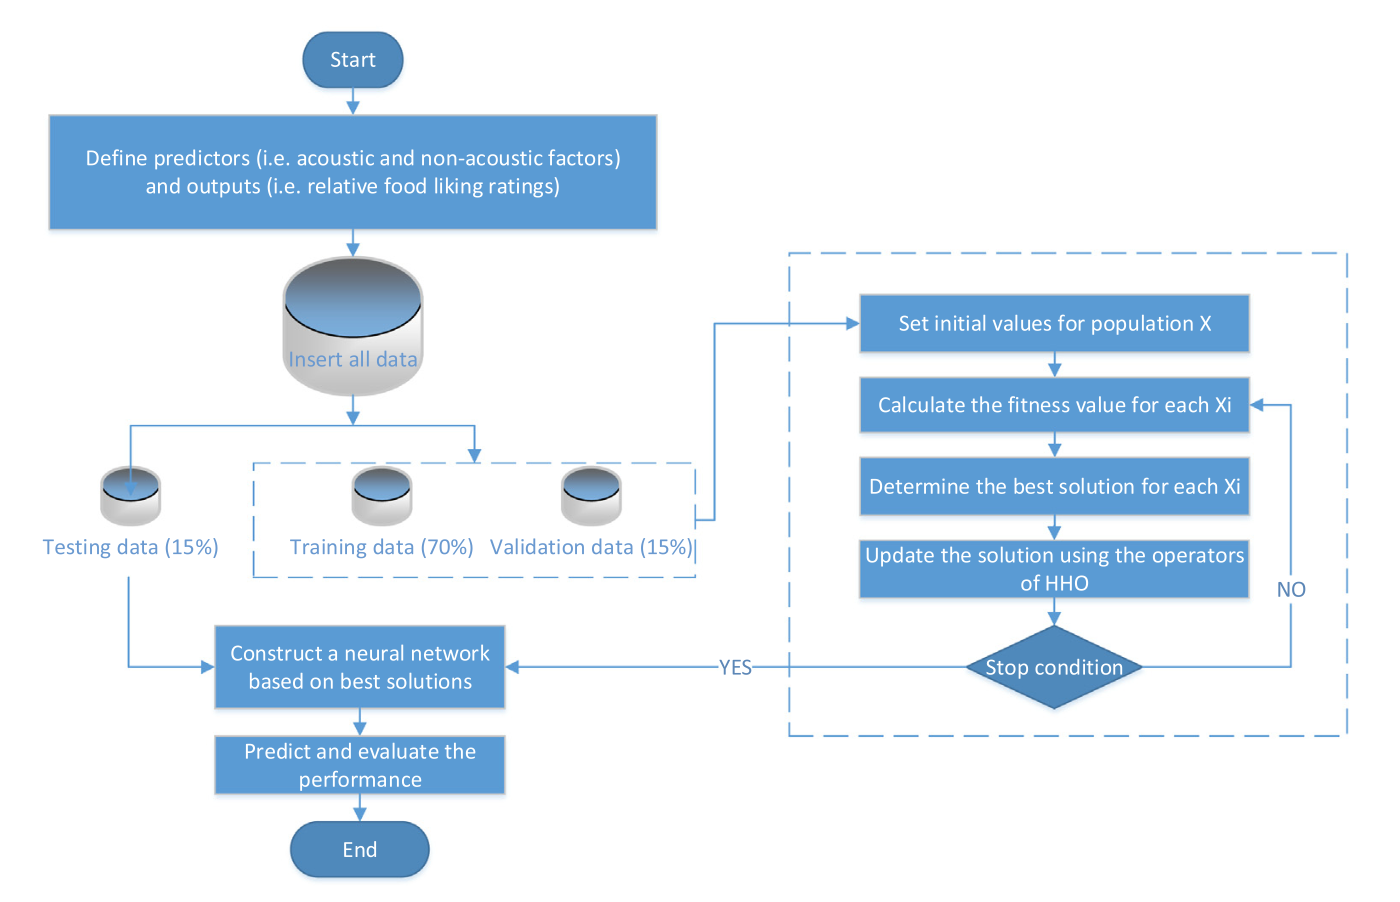
\includegraphics[width=0.7\textwidth]{Chapters/Figures/HHO-ANN.png}
      \caption{Il modello HHO-ANN proposto per la previsione del gradimento del cibo, in relazione al rumore di fondo nell'ambiente di ascolto. \cite{alamir2021enhanced}}
      \label{hho-ann}
\end{figure}

Grazie alla sua architettura avanzata e all'utilizzo dell'ottimizzazione \gls{hho}, il modello ANN-HHO è risultato altamente efficace nel prevedere la gradevolezza relativa del cibo in presenza di diversi tipi e livelli di rumore di fondo, fornendo uno strumento prezioso per comprendere e mitigare l'impatto acustico nel settore ristorativo.

\section{Risultati e analisi delle prestazioni}
\noindent

Presentiamo i risultati del modello ANN-HHO e confronta le sue prestazioni con quelle dei modelli \gls{ann} tradizionali (i \gls{ffnn}) e dei modelli statistici misti.

Il confronto delle prestazioni del modello è riportato di seguito:

\begin{itemize}
      \item \textbf{Modello \gls{ffnn} ordionario:}
            \begin{itemize}
                  \item RMSE = 1.1
                  \item MSE = 1.1
                   \item MAE = 0.8
            \end{itemize}       
\end{itemize}

\begin{figure}[H]
      \captionsetup{font=scriptsize}
      \centering
      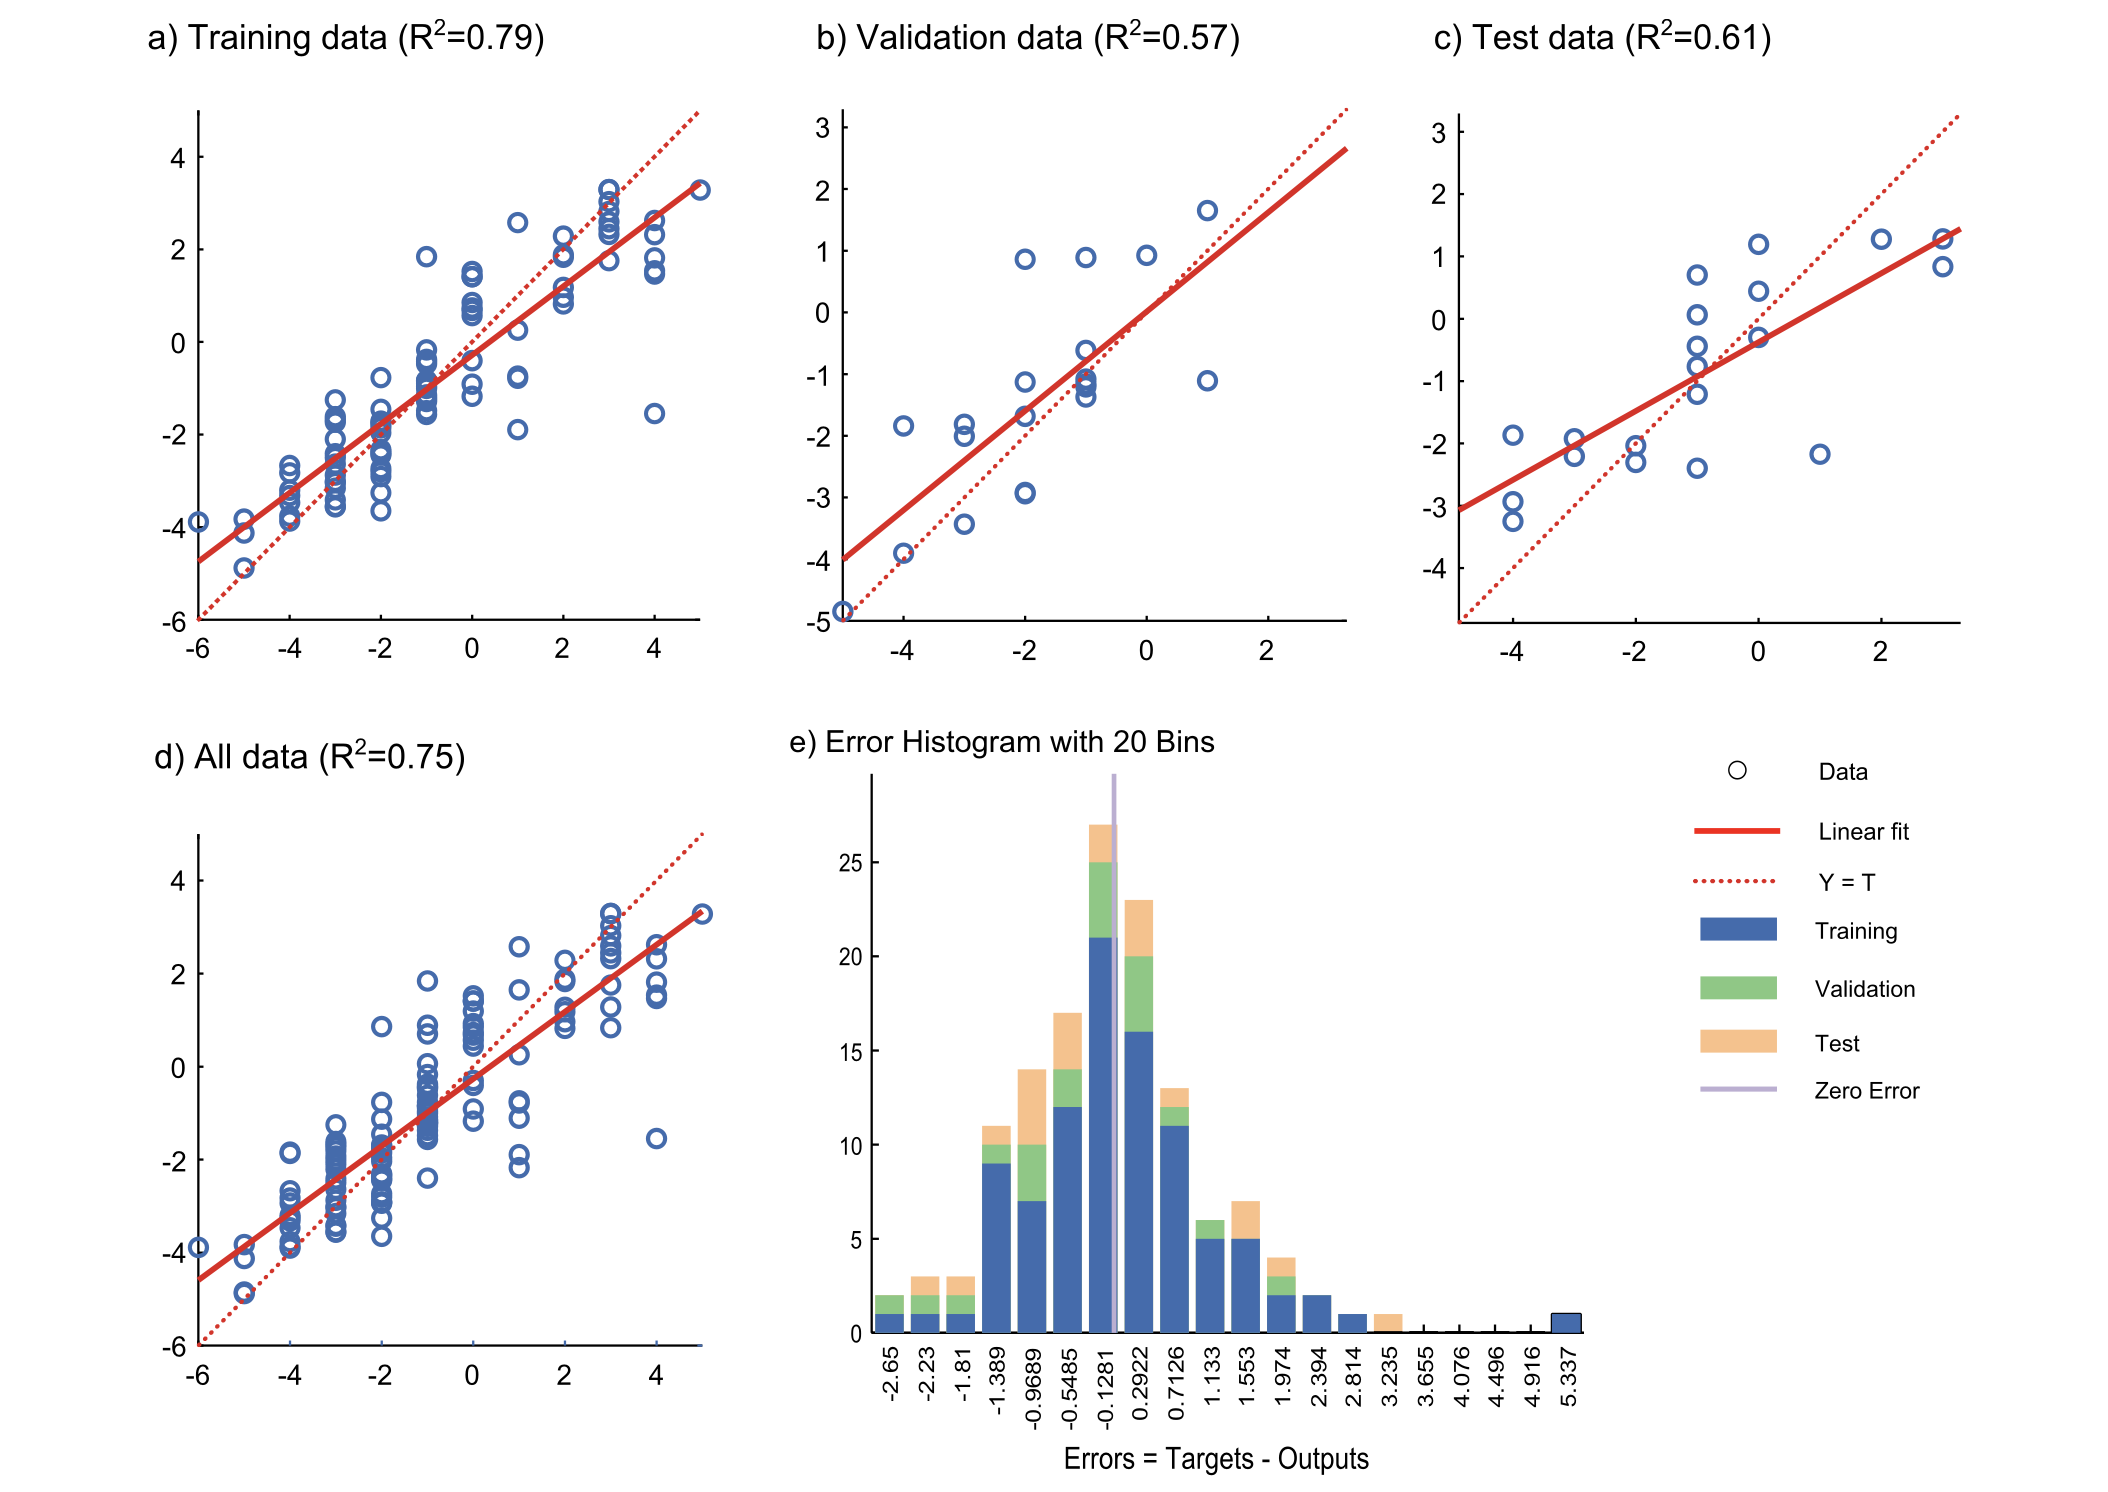
\includegraphics[width=1\textwidth]{Chapters/Figures/ffnn-result.png} 
      \caption{\small Le prestazioni delle reti neurali feedforward ordinarie per la previsione del gradimento relativo degli alimenti (FFNN). La correlazione tra i valori mirati del gradimento relativo del cibo (sull'asse delle ascisse) e i valori previsti del gradimento relativo del cibo (sull'asse delle ordinate) sono mostrati per (a) i dati di formazione (b) i dati di convalida (c) i dati di prova (d) tutti i dati. I residui per i dati di formazione, convalida e test sono mostrati nella parte (e). \cite{alamir2021enhanced}}
      \label{fig:ffnn-abc}
\end{figure}

\newpage
\begin{itemize}
       \item \textbf{Modello ANN-HHO:}
            \begin{itemize}
                  \item RMSE = 0.8
                  \item MSE = 0.6
                  \item MAE = 0.7
            \end{itemize}
\end{itemize}

\begin{figure}[H]
      \captionsetup{font=scriptsize}
      \centering
      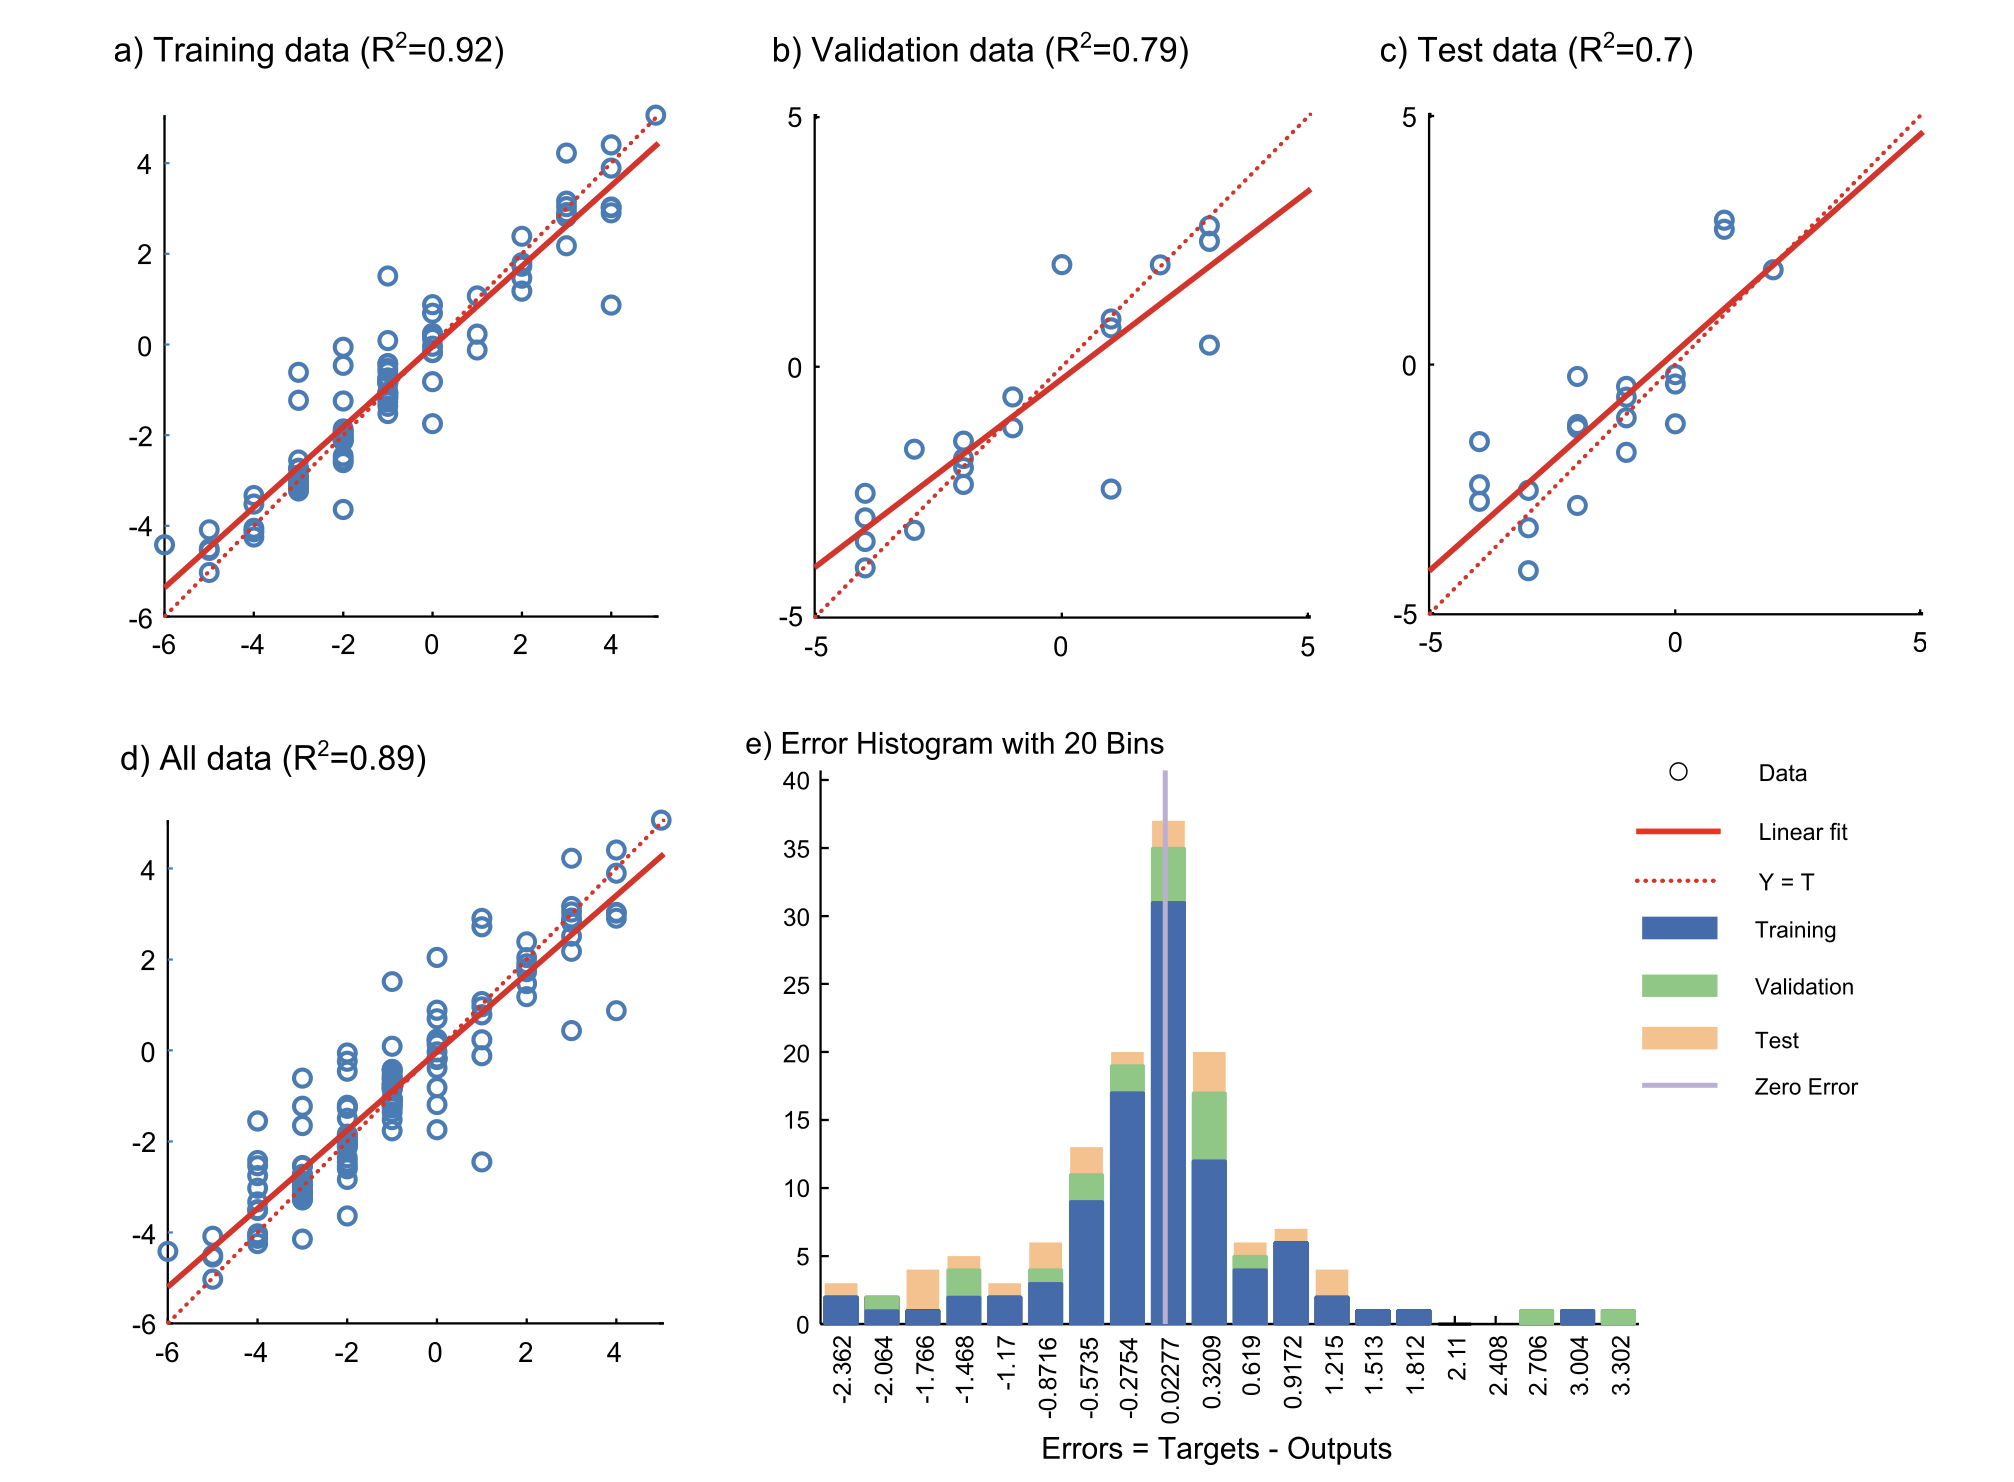
\includegraphics[width=1\textwidth]{Chapters/Figures/ann-hho-result.png} 
      \caption{\small Le prestazioni della rete neurale potenziata che utilizza l'ottimizzatore di Harris Hawks (ANN-HHO). La correlazione tra i valori mirati del gradimento relativo del cibo (sull'asse delle ascisse) e i valori previsti del gradimento relativo del cibo (sull'asse delle ordinate) sono mostrati per (a) i dati di formazione (b) i dati di convalida (c) i dati di prova (d) tutti i dati. I residui per i dati di formazione, convalida e test sono mostrati nella parte (e). \cite{alamir2021enhanced}}
      \label{fig:ann-hho-abc}
\end{figure}

\begin{itemize}
      \item \textbf{Modello statistico misto:}
            \begin{itemize}
                  \item R\textsuperscript{2} = 0.42
                  \item RMSE = 1.8
            \end{itemize}
\end{itemize}

Quindi il modello ANN-HHO ha mostrato la migliore accuratezza nella previsione delle valutazioni relative di gradevolezza del cibo, rispetto ai modelli \gls{ffnn} tradizionali e al modello misto.

\begin{comment}

\begin{figure}[H]
      \centering
      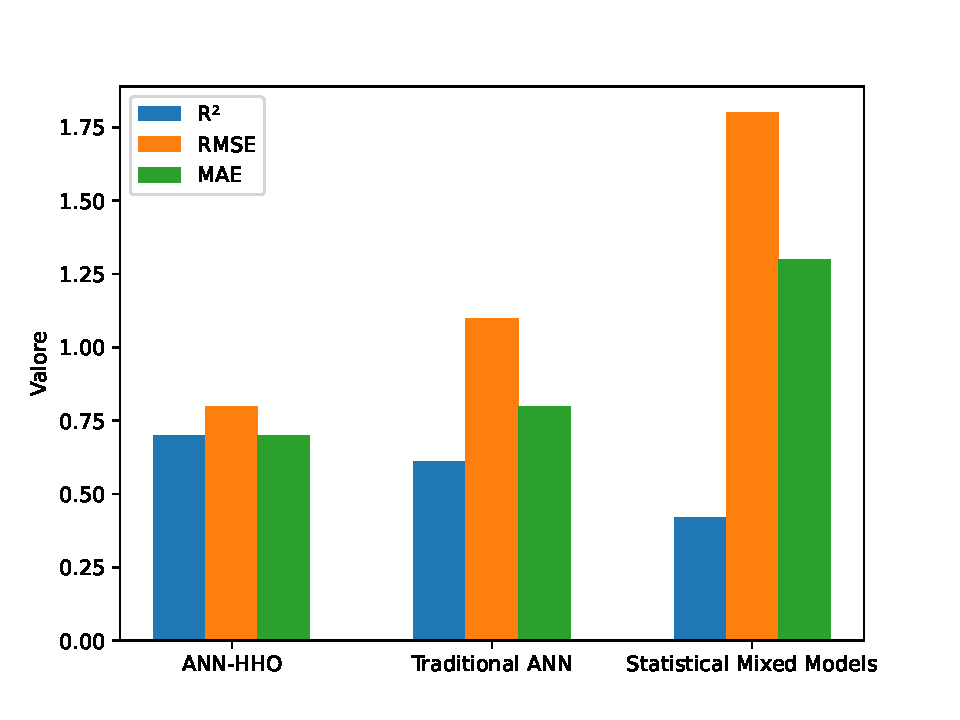
\includegraphics[width=0.7\textwidth]{Chapters/Figures/grafico_performance_modelli.pdf}
      \caption{\small Confronto delle prestazioni di ANN-HHO, ANN tradizionale e modelli statistici misti per la previsione del gradimento dei cibi. Il grafico mostra l'R-quadrato (R²), l'errore quadratico medio (RMSE) e l'errore assoluto medio (MAE) per ciascun modello, dimostrando la superiorità delle prestazioni dell'approccio ANN-HHO.}
      \label{fig:graph_label}
\end{figure}

\end{comment}

\begin{comment}

I risultati principali del modello ANN-HHO includono:

\begin{itemize}
    \item \textbf{Livelli ottimali di rumore:} Il modello prevede il massimo gradimento relativo del cibo a livelli di rumore compresi tra 30 e 35 dBA per diversi tipi di rumore.
    
    \item \textbf{Impatto del tipo di rumore:}
    \begin{itemize}
        \item \textit{Musica:} Impatto positivo sul gradimento del cibo fino a 47 dBA.
        \item \textit{Rumore dei ristoranti e del traffico stradale:} Impatto negativo a tutti i livelli studiati.
    \end{itemize}
    
    \item \textbf{Analisi delle soglie:}
    \begin{itemize}
        \item \textit{Musica e rumore del ristorante:} 30 dBA per il massimo gradimento.
        \item \textit{Rumore del traffico stradale:} 35 dBA per il massimo gradimento.
    \end{itemize}
\end{itemize}

\end{comment}


\newpage
La figura \ref{fig:prediction_food} mostra i risultati delle previsioni del modello ANN-HHO sulla gradevolezza relativa del cibo a diversi livelli di rumore per i tre tipi di rumore testati.

\begin{figure}[H]
      \centering
      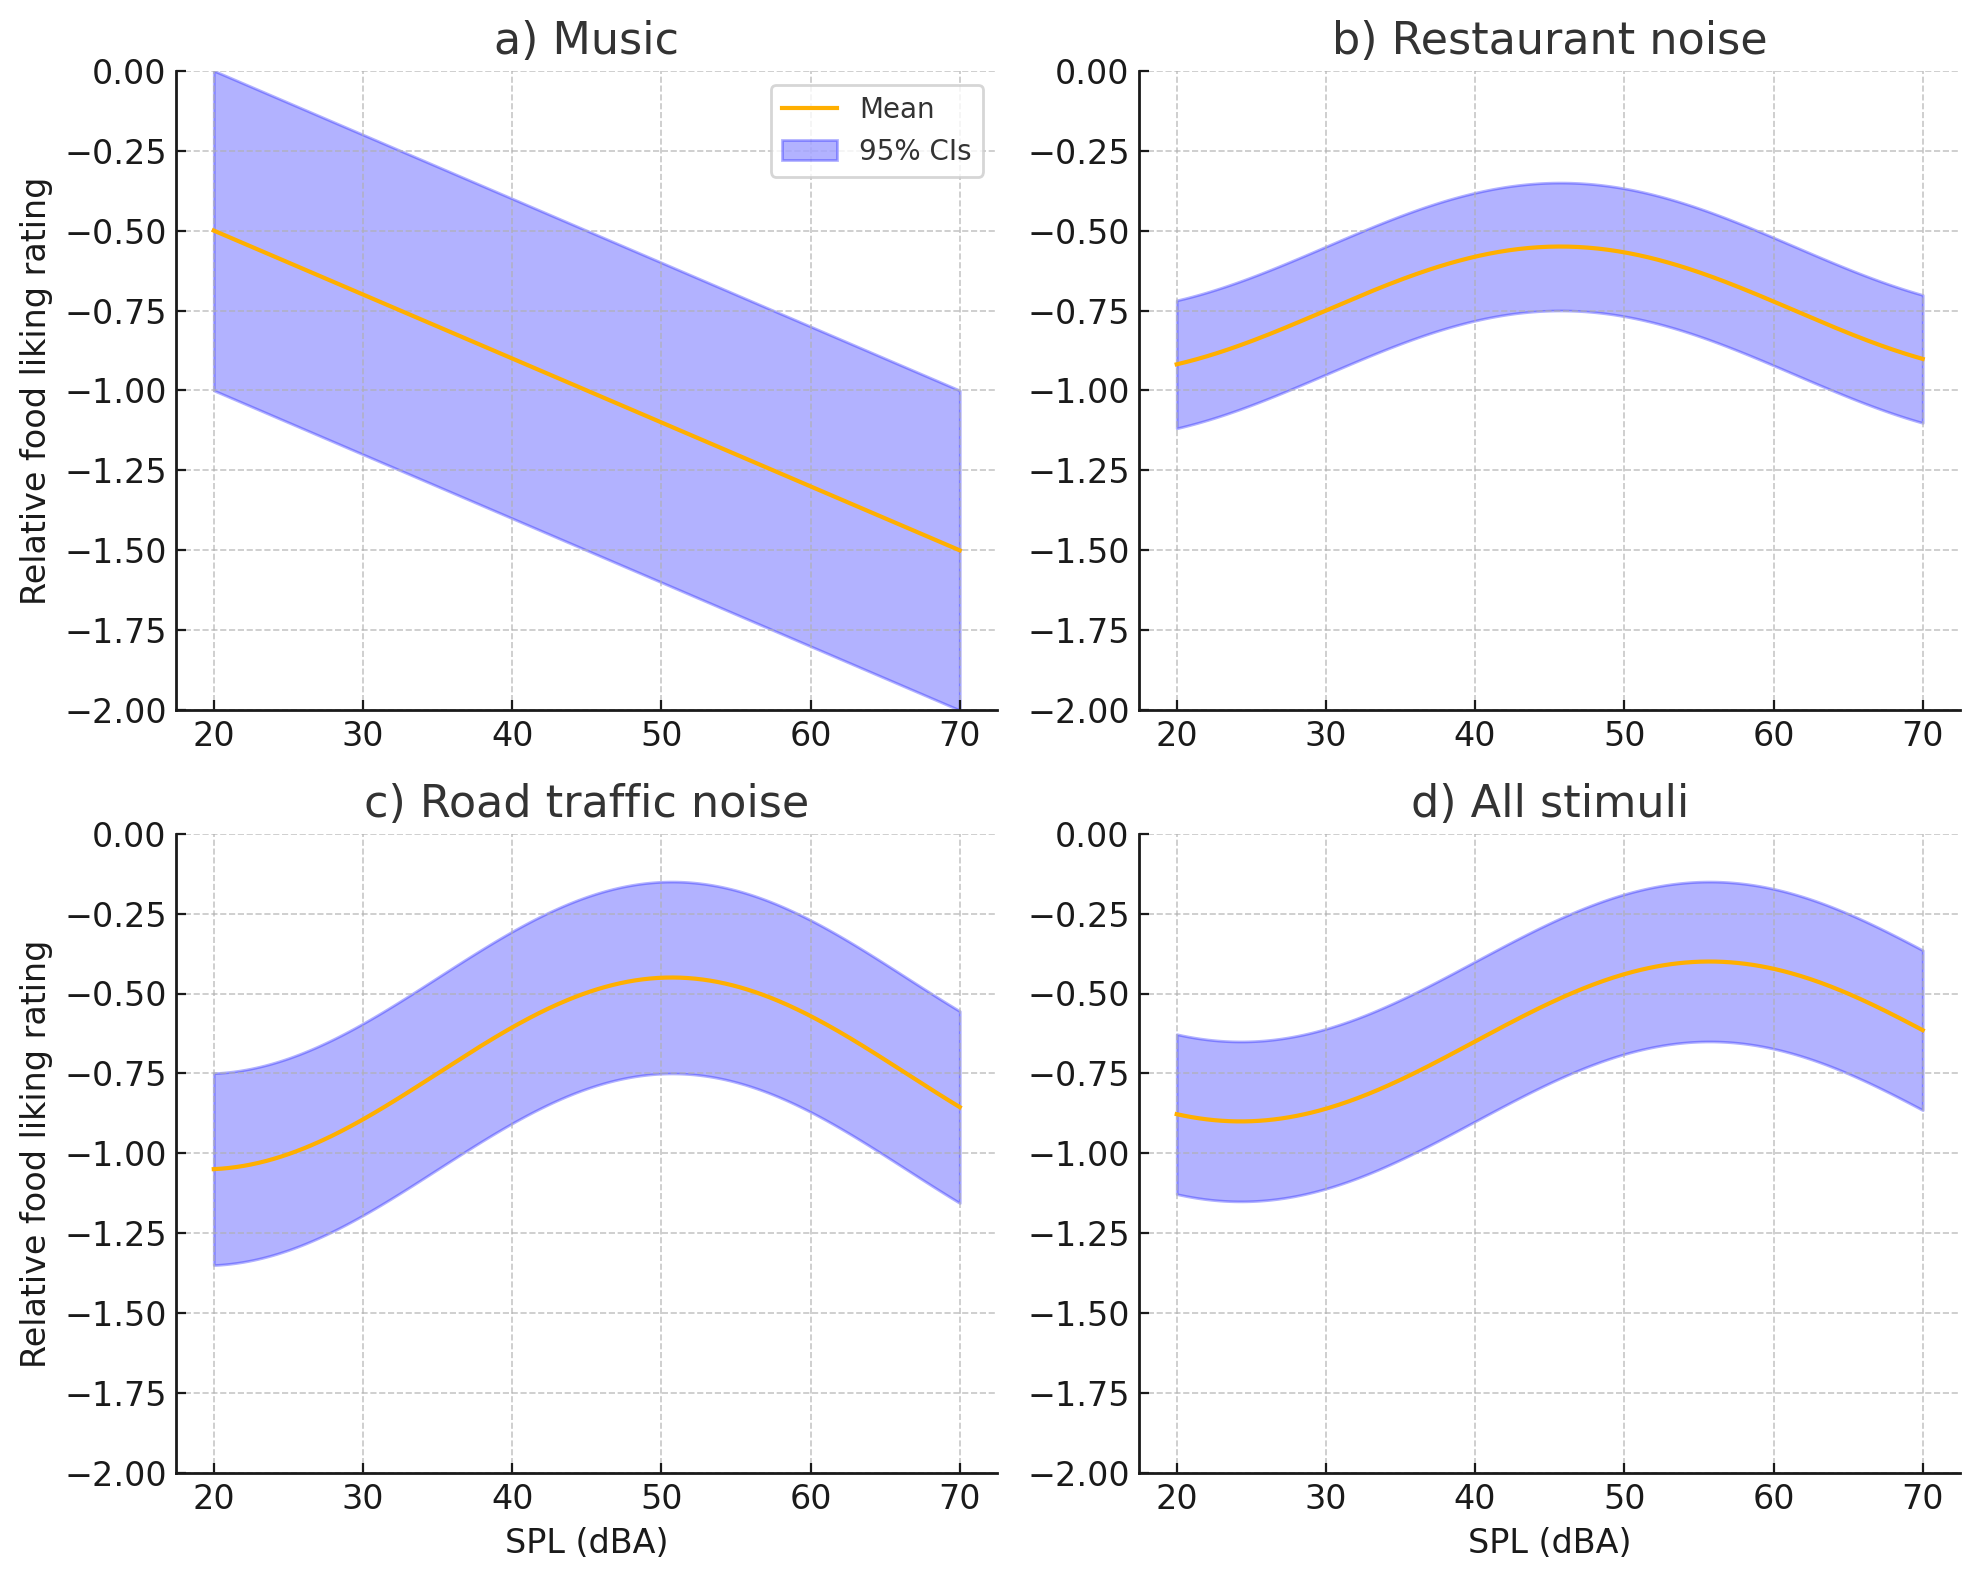
\includegraphics[width=0.7\textwidth]{Chapters/Figures/prediction_food.png}
      \caption{\small Previsione del gradimento relativo del cibo a diversi livelli utilizzando la ANN-HHO potenziata per a) musica b) rumore del ristorante c) rumore del traffico stradale e d) tutti gli stimoli acustici. Le linee solide indicano la media e le linee blu ombreggiate indicano le 95{\%} CIs associate alla media.}
      \label{fig:prediction_food}
\end{figure}

I risultati ottenuti indicano che il modello ANN-HHO ha raggiunto prestazioni superiori rispetto ai modelli tradizionali nella previsione del gradimento alimentare in presenza di rumore di fondo. In particolare, l'analisi dei diversi tipi di rumore mostra come specifici livelli influenzino la gradevolezza percepita del cibo in modo significativo.

Per il sottofondo musicale, il modello prevede che un livello intorno ai 30 dBA sia quello che massimizza la gradevolezza relativa del cibo, con una tendenza a diminuire man mano che il livello del rumore supera questa soglia.

Anche per il rumore caratteristico degli ambienti ristorativi, la previsione indica che 30 dBA rappresenta la soglia di massima gradevolezza, seguita da un calo con l'aumento dell'intensità sonora.

Una dinamica simile è osservata per il rumore del traffico stradale, dove il livello di 35 dBA porta alla massima percezione di gradimento del cibo, seguito anche in questo caso da un decremento in relazione all'aumento del rumore.

Considerando i risultati complessivi per tutti i tipi di rumore, il modello suggerisce che il livello di rumore ottimale per una gradevolezza relativa media più alta si attesti intorno ai 30 dBA. Questo valore rappresenta il punto in cui la percezione del gradimento è massimizzata, confermando come livelli sonori moderati, piuttosto che elevati, possano influire positivamente sull'esperienza gustativa in ambienti di ristorazione.

È importante notare che i valori massimi sono stati determinati attraverso una rappresentazione continua delle previsioni, quindi i valori vicini non differivano in modo significativo.

\begin{figure}[H]
      \centering
      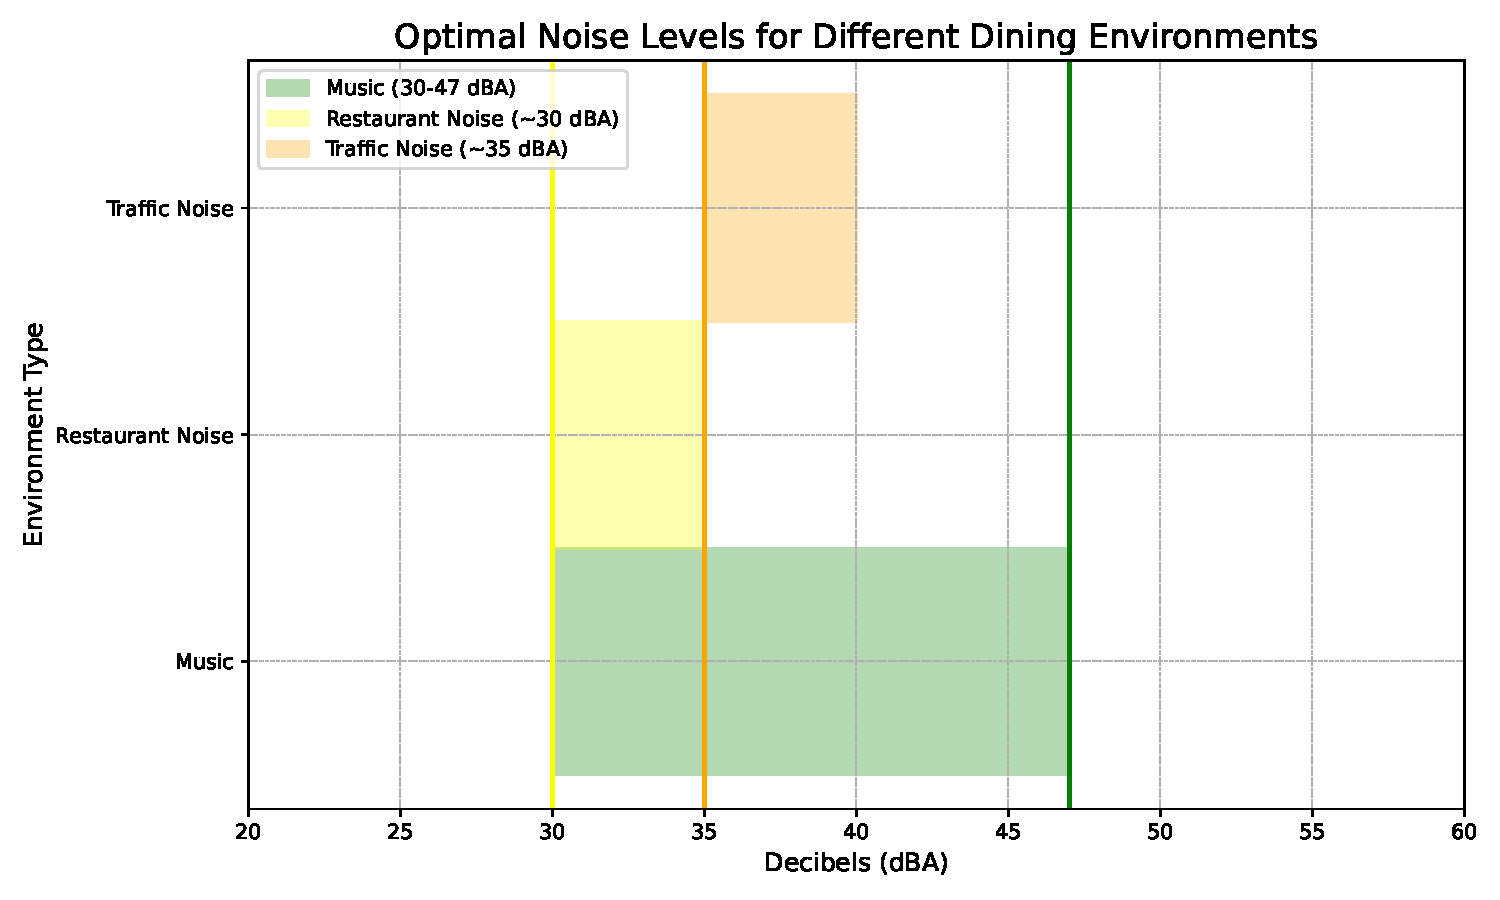
\includegraphics[width=0.7\textwidth]{Chapters/Figures/optimal_noise_levels_improved.pdf} % Specifica il percorso corretto del tuo file PDF
      \caption{\small Livelli di rumorosità ottimali per i diversi ambienti di ristorazione}
      \label{fig:graph_label}
\end{figure}

\begin{comment}

\section{Applicazione del modello alla previsione del gradimento del cibo}
\noindent

Questa sezione esplora le implicazioni pratiche e le intuizioni derivate dalle previsioni del modello ANN-HHO per il gradimento del cibo in vari ambienti acustici. \\
\textbf{Ottimizzazione dell'ambiente acustico:} \\
Sulla base delle previsioni del modello, possiamo proporre delle linee guida per un ambiente acustico ottimale nelle aree di ristorazione:
\begin{enumerate}
    \item \textbf{Intervallo di rumore ideale:} Mantenere i livelli di rumore di fondo tra 30-35 dBA per ottimizzare il gradimento del cibo in diversi tipi di rumore.
    \item \textbf{Selezione della musica:} Quando si usa la musica di sottofondo, si possono tollerare livelli fino a 47 dBA senza un impatto negativo significativo sul gradimento del cibo.
    \item \textbf{Attenuazione del rumore:} È necessario prestare particolare attenzione alla riduzione del traffico stradale e del rumore generale dei ristoranti, poiché questi hanno effetti negativi più pronunciati anche a livelli più bassi.
\end{enumerate}

\textbf{Personalizzazione dell'esperienza culinaria:} \\
La capacità del modello di tenere conto dei fattori individuali consente di fornire raccomandazioni personalizzate:
\begin{enumerate}
    \item \textbf{Considerazioni basate sull'età:} Anche se l'età è risultata essere meno influente, si potrebbero prendere in considerazione dei leggeri aggiustamenti dei livelli di rumore per i diversi gruppi di età.
    \item \textbf{Preferenze specifiche di genere:} Il modello suggerisce lievi variazioni nella tolleranza al rumore tra i due sessi, che potrebbero essere prese in considerazione per la disposizione dei posti a sedere o la suddivisione in zone acustiche dei ristoranti.
    \item \textbf{Adattamento della sensibilità:} Per i clienti con un'elevata sensibilità al rumore, il modello raccomanda un'aderenza più rigorosa all'estremità inferiore dell'intervallo di rumore ottimale.
\end{enumerate}

\textbf{Strategie pratiche di attuazione:}
\begin{enumerate}
    \item \textbf{Zonizzazione acustica:} Progettare i ristoranti con zone acustiche distinte per soddisfare le diverse preferenze e sensibilità.
    \item \textbf{Controllo dinamico del rumore:} Implementare sistemi audio intelligenti che regolano i livelli di rumore in base all'ora del giorno, all'occupazione e ai profili dei clienti.
    \item \textbf{Formazione del personale:} Istruire il personale del ristorante sull'importanza dell'ambiente acustico e su come gestirlo in modo efficace.
\end{enumerate}

% Figure: Conceptual Design of Acoustically Optimized Dining Area [Create a new figure showing a restaurant floor plan with different acoustic zones]%

Queste applicazioni pratiche dimostrano come le intuizioni del modello ANN-HHO possano essere tradotte in strategie attuabili per migliorare le esperienze di ristorazione attraverso l'ottimizzazione dell'ambiente acustico. Considerando sia le tendenze generali sia i fattori individuali, i ristoranti e i locali possono creare atmosfere più piacevoli e personalizzate per i loro clienti.

\end{comment}

\section{Discussione e implicazioni}
\noindent

I risultati hanno dimostrato che il rumore di fondo può influenzare in modo significativo la gradevolezza percepita del cibo, a seconda del tipo e del livello di rumore presente.

Il modello ANN-HHO ottimizzato è stato quindi utilizzato per prevedere i livelli di rumore che massimizzano la gradevolezza relativa del cibo per i tre tipi di rumore testati. I risultati hanno mostrato che i livelli tra 30 dBA e 35 dBA davano la gradevolezza relativa massima, nonostante il rumore del traffico stradale e il rumore del ristorante diminuissero la gradevolezza a tutti i livelli. La musica, invece, poteva essere preferibile fino a 47 dBA.

\begin{figure}[H]
      \centering
      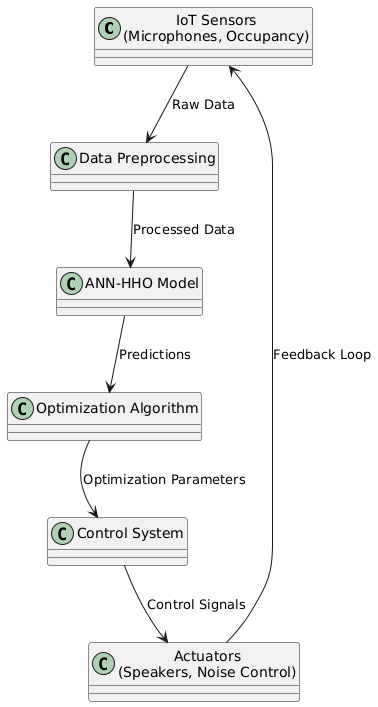
\includegraphics[width=0.4\textwidth]{Chapters/Figures/real_time_system.png}
      \caption{\small Proposed Framework for Real-time Acoustic Optimization System integrating ANN-HHO model.}
      \label{fig:realtimesystem}
\end{figure}

Questa ricerca contribuisce al campo dell'ingegneria dimostrando l'efficacia dei modelli ibridi di intelligenza artificiale nella risoluzione di problemi complessi del mondo reale. Il modello ANN-HHO non solo fornisce previsioni accurate ma offre anche interpretabilità, risolvendo una critica comune alle reti neurali. Il successo dell'applicazione nell'ottimizzazione dell'ambiente acustico apre nuove strade all'IA nella progettazione esperienziale e nella ricerca sensoriale.

I risultati pongono le basi per lo sviluppo di sistemi intelligenti in grado di regolare l'ambiente in tempo reale, rivoluzionando potenzialmente l'approccio alla progettazione acustica degli spazi pubblici. Il lavoro futuro dovrebbe concentrarsi sull'espansione delle capacità del modello, sull'esplorazione di integrazioni multimodali e sullo studio della sua scalabilità in diversi contesti.
